\section{Introduction}
I have spent the majority of my time this week trying to finish the EPFL Deep Learning Course EE559 as well as doing the miniproject number 1 from EPFL\cite{miniproject1}.

\section{EPFL Deep Learning Course}
This week I continued learning the EPFL course and I finished 2 more lectures. They were all complex but once I achieved the key ideas they turned out to be very fascinating.

\textbf{\emph{Going deeper}}. The lecturer taught me about rectifiers (ReLU), drop-out, batch normalization in theory and practical, the architecture of residual networks, some tips to gain good results in training state such as advanced weight initialization. The lecturer also taught me about differences in perform-ance of GPU and CPU, programming techniques with torch.cuda in PyTorch.

\textbf{\emph{Computer vision}}. The lecturer taught me about architectures of Deep networks for image classification such as AlexNet, VGGNet\cite{vggnet}; object detection algorithm YOLO\cite{yolo}, and semantic segmentation (FCN)\cite{semanticseg}, data-loaders, fine-tuning and neuro-surgery.

I had updated the taken notes and all of them could be found \href{https://gitlab.com/tlvu2697/epfl--ee559--deep-learning}{here on my GitLab}.

\section{Mini-project 1}
Beside learning materials from course, I also tried implementing the mini-project 1 to gain more practical experience. The objective of this project was to train a predictor of finger movements from Electroencephalography (EEG) recordings\cite{eegrecord}. The data and other materials also be provided by the course to help me understanding and doing the project better.

\subsection{Problems}
At the beginning, I made a big mistake that prevent me from achieving any goals which was using the Sigmoid function at the last layer of my CNN architecture. After days of training with all of my effort, the network did not gain anything and the loss was still a huge number. After searching on the internet and asking experience from my friend I figured out the problem. I fixed the architecture later and the network seemed to work well also.

\subsection{Architecture}
The data composed of 316 training recordings, and 100 test recordings, each composed of 28 EEG channels sampled at 1khz for 0.5s. Concretely, the train dataset had the shape of [316, 28, 50] and the test dataset has the shape of [100, 28, 50]. After examining the structure of dataset I started designing the appropriate Convolutional Neural Network. I tried to increase the channel from 28 to 56, then to 112 by two 1d convolutional layer and apply max pooling after each convolutional layer. After the two convolutional layers the shape of data was [316, 112, 2]. Then I chose the nb-hidden of 100 and two fully-connected layer. Finally the output of my network was 2 numbers for classification purpose. I also used CrossEntropyLoss loss and SGD optimizer during my training process.

\begin{figure}[!ht]
\centering
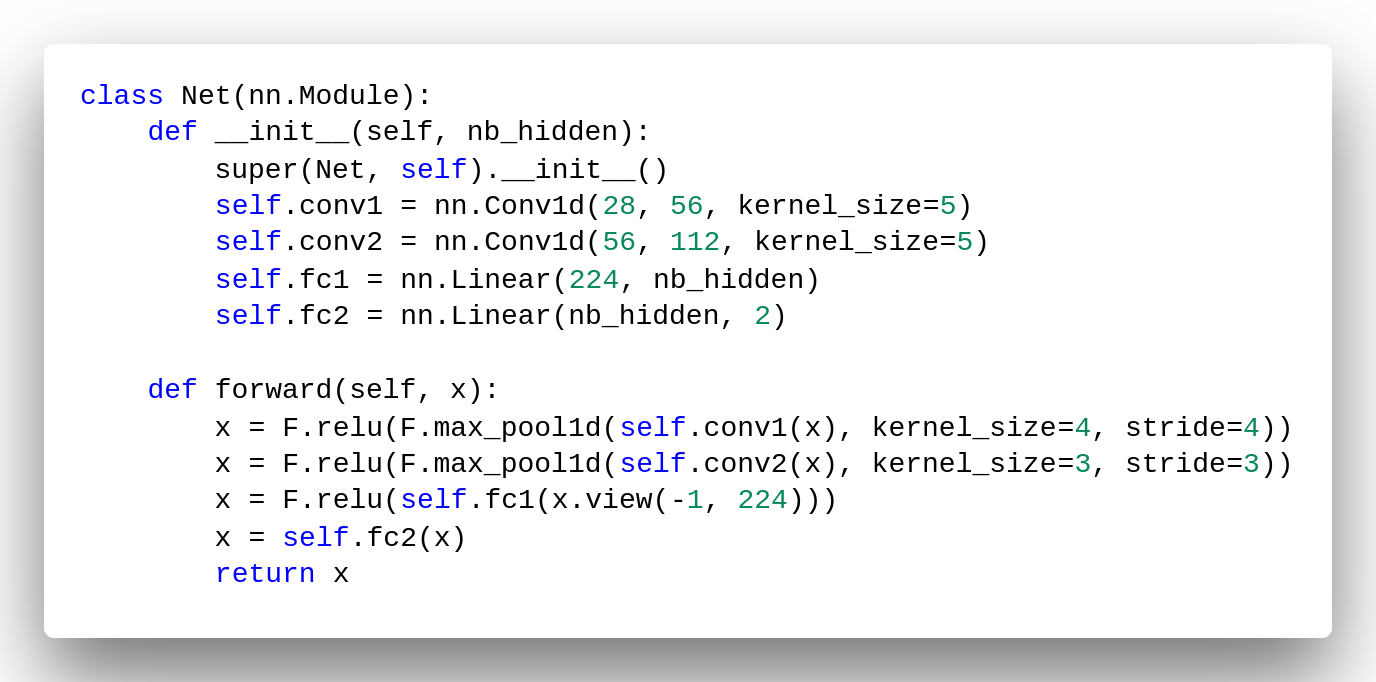
\includegraphics[width=\textwidth,keepaspectratio]{week2-mini-project-1-net.png}
\caption{Convolutional Neural Network architecture}
\end{figure}


\subsection{Goals}
With the learning rate of 1e-3 and after 5000 epochs. I got the train error of 0\% (0/316) and the test error of 36\% (36/100).

I also tried to apply dropout layer to my CNN architecture but the result was not change significantly. Maybe dropout layer had no effect on my CNN architecture, or I did not use it in the right way though. There was one thing that I was not try, the batch processing technique, I perhaps should try it later on my next convolutional neural networks. 

\subsection{Source code}
All of my work could be found \href{https://gitlab.com/tlvu2697/epfl--ee559--deep-learning/blob/master/practical/mini-project-1.py}{on my GitLab}.